%% AHHS

\section{Exercises}

%_________________
\subsection{Case study}
% 1.6.1

% 1

\eoce{\qt{Migraine and acupuncture}
A migraine is a particularly painful type of headache, which patients sometimes wish to treat with acupuncture. To determine whether acupuncture relieves migraine pain, researchers conducted a completely randomized controlled study where 89 females diagnosed with migraine headaches were randomly assigned to one of two groups: treatment or control. 43 patients in the treatment group received acupuncture that is specifically designed to treat migraines. 46 patients in the control group received placebo acupuncture (needle insertion at nonacupoint locations). 24 hours after patients received acupuncture, they were asked if they were pain free. Results are summarized in the contingency table below. \footfullcite{Allais:2011}

\noindent\begin{minipage}[l]{0.4\textwidth}
\begin{tabular}{ll  cc c} 
			&				& \multicolumn{2}{c}{\textit{Pain free}} \\
\cline{3-4}
			&							& Yes 	& No 	& Total	\\
\cline{2-5}
							&Treatment 	& 10	 	& 33		& 43 	\\
\raisebox{1.5ex}[0pt]{\emph{Group}}	& Control		& 2	 	& 44 	 	& 46 \\
\cline{2-5}
							&Total		& 12		& 77		& 89
\end{tabular}
\end{minipage}
\begin{minipage}[c]{0.05\textwidth}
\end{minipage}
\begin{minipage}[c]{0.27\textwidth}
\begin{center}
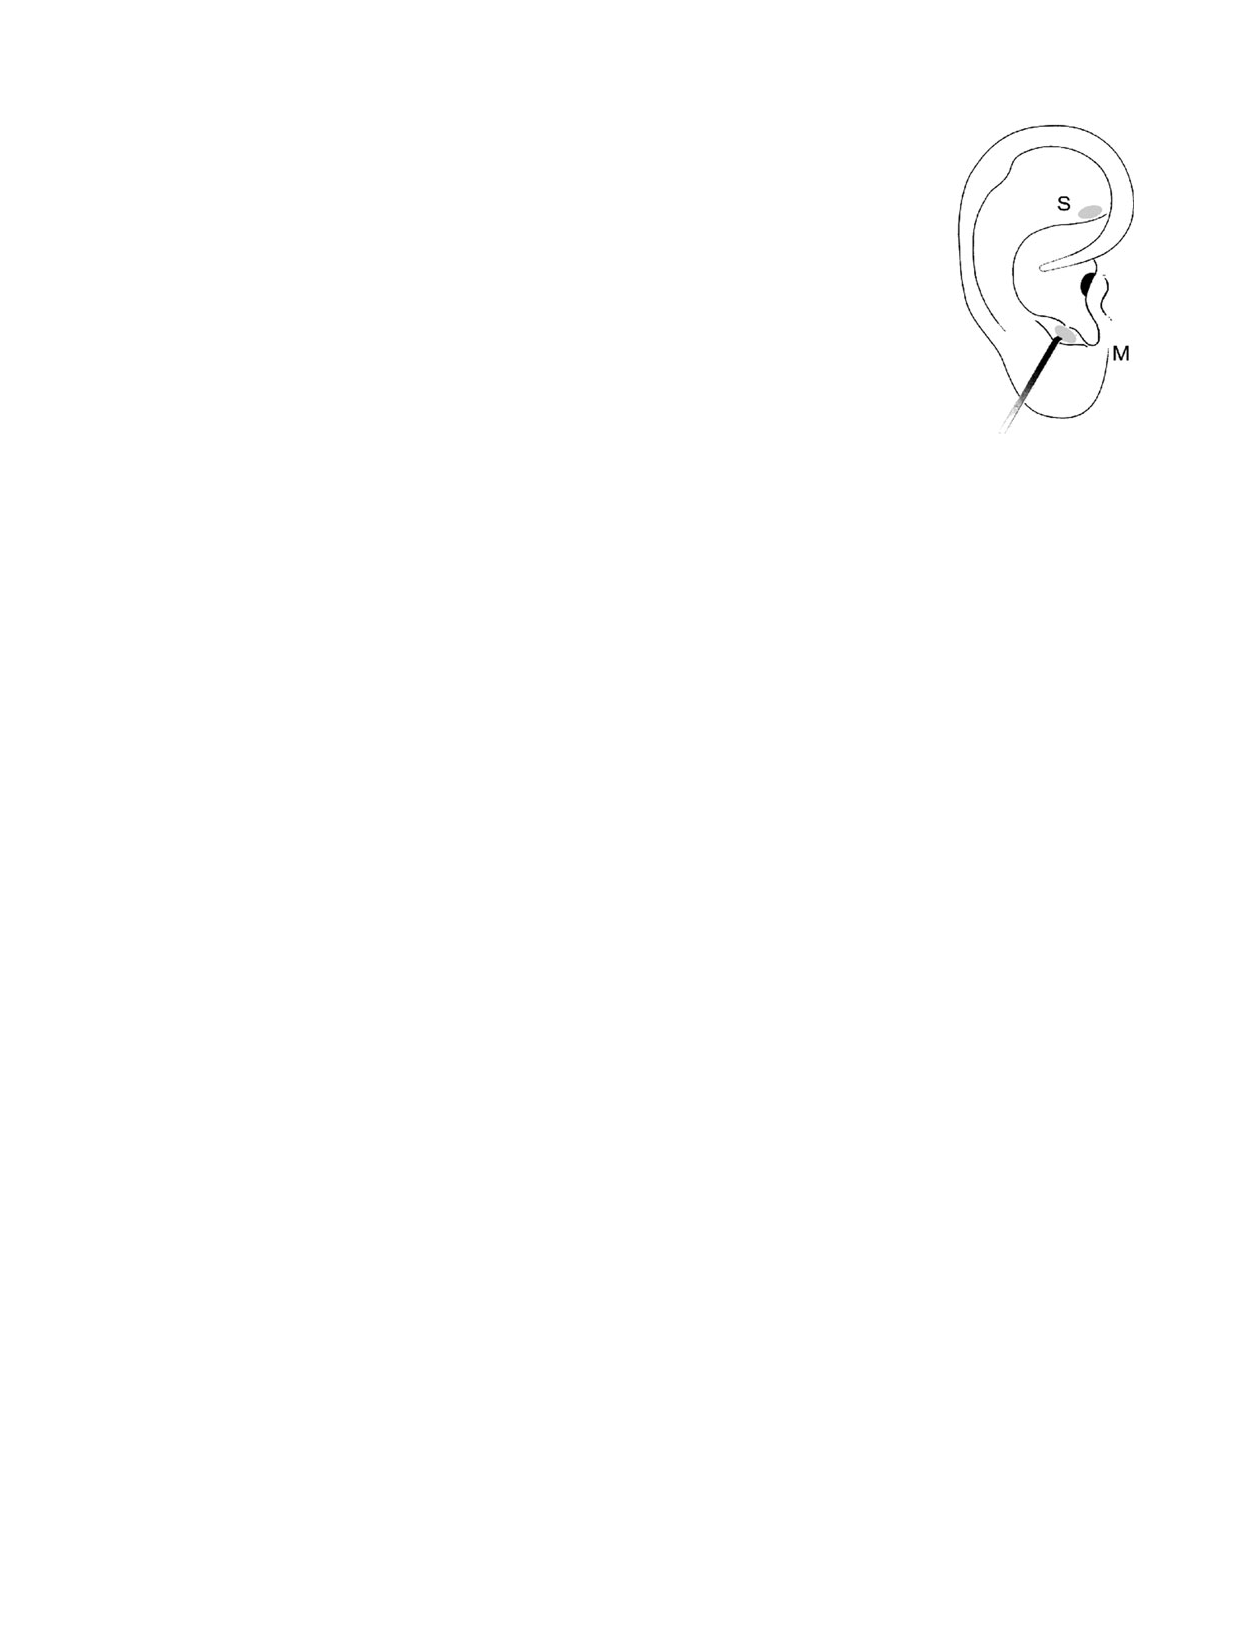
\includegraphics[width = 0.75\textwidth]{ch_data_collection/figures/eoce/images/earacupuncture}
\end{center}
\end{minipage}
\begin{minipage}[c]{0.25\textwidth}
{\footnotesize Figure from the original paper displaying the appropriate area (M) versus the inappropriate area (S) used in the treatment of migraine attacks.}
\end{minipage}
\begin{parts}
\item What percent of patients in the treatment group were pain free 24 hours after receiving acupuncture? What percent in the control group?
\item Based on your findings in part~(a), which treatment appears to be more effective for migraines?
\item Do the data provide convincing evidence that there is a real pain reduction for those patients in the treatment group? Or do you think that the observed difference might just be due to chance?
\end{parts}
}
{}

% 2

\eoce{\qt{Sinusitis and antibiotics, Part I\label{sinusitis}} Researchers studying the effect of antibiotic treatment for acute sinusitis compared to symptomatic treatments randomly assigned 166 adults diagnosed with acute sinusitis to one of two groups: treatment or control. Study participants received either a 10-day course of amoxicillin (an antibiotic) or a placebo similar in appearance and taste. The placebo consisted of symptomatic treatments such as acetaminophen, nasal decongestants, etc. At the end of the 10-day period patients were asked if they experienced significant improvement in symptoms. The distribution of responses are summarized below. \footfullcite{Garbutt:2012}
\begin{center}
\begin{tabular}{ll  cc c} 
			&				& \multicolumn{2}{c}{\textit{Self-reported significant}} \\
			&				& \multicolumn{2}{c}{\textit{improvement in symptoms}} \\
\cline{3-4}
			&							& Yes 	& No 	& Total	\\
\cline{2-5}
							&Treatment 	& 66	 	& 19		& 85 	\\
\raisebox{1.5ex}[0pt]{\emph{Group}}	& Control		& 65	 	& 16 	 	& 81 \\
\cline{2-5}
							&Total		& 131	& 35		& 166
\end{tabular}
\end{center}
\begin{parts}
\item What percent of patients in the treatment group experienced a significant improvement in symptoms? What percent in the control group?
\item Based on your findings in part (a), which treatment appears to be more effective for sinusitis?
\item Do the data provide convincing evidence that there is a difference in the improvement rates of sinusitis symptoms? Or do you think that the observed difference might just be due to chance?
\end{parts}
}
{}


%_________________
\subsection{Data basics}
% 1.6.2

% 3

\eoce{\qt{Identify study components, Part I\label{components1}} Identify (i) the cases, (ii) the variables and their types, and (iii) the main research question in the studies described below.
\textA{\vspace{2mm}}
\begin{parts}
\item Researchers collected data to examine the relationship between pollutants and preterm births in Southern California. During the study air pollution levels were measured by air quality monitoring stations. Specifically, levels of carbon monoxide were recorded in parts per million, nitrogen dioxide and ozone in parts per hundred million, and coarse particulate matter (PM$_{10}$) in $\mu g/m^3$. Length of gestation data were collected on 143,196 births between the years 1989 and 1993, and air pollution exposure during gestation was calculated for each birth. The analysis suggested that increased ambient PM$_{10}$ and, to a lesser degree, CO concentrations may be associated with the occurrence of preterm births. \footfullcite{Ritz+Yu+Chapa+Fruin:2000}
\textA{\vspace{2mm}}
\item The Buteyko method is a shallow breathing technique developed by Konstantin Buteyko, a Russian doctor, in 1952. Anecdotal evidence suggests that the Buteyko method can reduce asthma symptoms and improve quality of life. In a scientific study to determine the effectiveness of this method, researchers recruited 600 asthma patients aged 18-69 who relied on medication for asthma treatment. These patients were split into two research groups: one practiced the Buteyko method and the other did not. Patients were scored on quality of life, activity, asthma symptoms, and medication reduction on a scale from 0 to 10. On average, the participants in the Buteyko group experienced a significant reduction in asthma symptoms and an improvement in quality of life. \footfullcite{McDowan:2003}
\end{parts}
}{}

% 4

\eoce{\qt{Identify study components, Part II\label{components2}} Identify (i) the cases, (ii) the variables and their types, and (iii) the main research question of the studies described below.
\begin{parts}
\item Researchers studying the relationship between honesty, age and self-control conducted an experiment on 160 children between the ages of 5 and 15. Participants reported their age, sex, and whether they were an only child or not. The researchers asked each child to toss a fair coin in private and to record the outcome (white or black) on a paper sheet, and said they they would only reward children who report white. Half the students were explicitly told not to cheat and the others were not given any explicit instructions. In the no instruction group probability of cheating was found to be uniform across groups based on child's characteristics. In the group that was explicitly told to not cheat, girls were less likely to cheat, and while rate of cheating didn't vary by age for boys, it decreased with age for girls. \footfullcite{Bucciol:2011} \label{luck_cheat}
\item In a study of the relationship between socio-economic class and unethical behavior, 129 University of California undergraduates at Berkeley were asked to identify themselves as having low or high social-class by comparing themselves to others with the most (least) money, most (least) education, and most (least) respected jobs. They were also presented  with a jar of individually wrapped candies and informed that they were for children in a nearby laboratory, but that they could take some if they wanted. Participants completed unrelated tasks and then reported the number of candies they had taken. It was found that those in the upper-class rank condition took more candy than did those in the lower-rank condition. \footfullcite{Piff:2012}
\end{parts}
}{}

\textA{\pagebreak}

% 5
\eoce{\qt{Fisher's irises} Sir Ronald Aylmer Fisher was an English statistician, evolutionary biologist, and geneticist who worked on a data set that contained sepal length and width, and petal length and width from three species of iris flowers (\textit{setosa}, \textit{versicolor} and \textit{virginica}). There were 50 flowers from each species in the data set. \footfullcite{Fisher:1936} \\
\noindent\begin{minipage}[c]{0.5\textwidth}
\begin{parts}
\item How many cases were included in the data?
\item How many numerical variables are included in the data? Indicate what they are, and if they are continuous or discrete.
\item How many categorical variables are included in the data, and what are they? List the corresponding levels (categories).
\end{parts}
\end{minipage}
\begin{minipage}[c]{0.03\textwidth}
\ 
\end{minipage}
\begin{minipage}[c]{0.15\textwidth}
\begin{center}
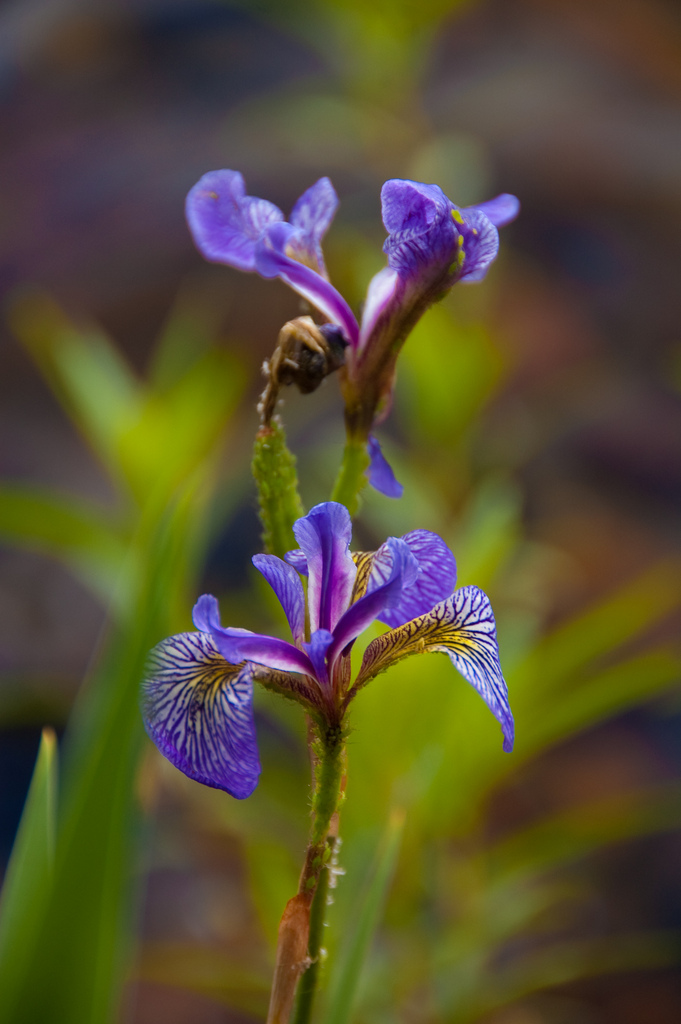
\includegraphics[width = \textwidth]{ch_data_collection/figures/eoce/images/irisversicolor}
\end{center}
\end{minipage}
\begin{minipage}[c]{0.01\textwidth}
\ 
\end{minipage}
\begin{minipage}[c]{0.25\textwidth}
{\raggedright\footnotesize Photo by Ryan Claussen (\oiRedirect{textbook-flickr_ryan_claussen_iris_picture}{http://flic.kr/p/6QTcuX}) \oiRedirect{textbook-CC_BY_SA_2}{CC~BY-SA~2.0~license}}\end{minipage}
}{}

% 6

\eoce{\qt{Smoking habits of UK residents\label{UKSmoking_datamatrix}} A survey was conducted to study the smoking habits of UK residents. Below is a data matrix displaying a portion of the data collected in this survey. Note that ``$\pounds$" stands for British Pounds Sterling, ``cig" stands for cigarettes, and ``N/A'' refers to a missing component of the data. \footfullcite{data:smoking}
\begin{center}
\scriptsize{
\begin{tabular}{rccccccc}
  \hline
 & sex & age & marital & grossIncome & smoke & amtWeekends & amtWeekdays \\ 
  \hline
1 & Female &  42 & Single & Under $\pounds$2,600 & Yes &  12 cig/day &  12 cig/day \\ 
2 & Male &  44 & Single & $\pounds$10,400 to $\pounds$15,600 & No & N/A & N/A \\ 
3 & Male &  53 & Married & Above $\pounds$36,400 & Yes &   6 cig/day &   6 cig/day \\ 
\vdots & \vdots &  \vdots & \vdots & \vdots & \vdots & \vdots & \vdots \\ 
1691 & Male &  40 & Single & $\pounds$2,600 to $\pounds$5,200 & Yes &   8 cig/day &   8 cig/day \\   
   \hline
\end{tabular}
}
\end{center}
\begin{parts}
\item What does each row of the data matrix represent?
\item How many participants were included in the survey?
\item Indicate whether each variable in the study is numerical or categorical. If numerical, identify as continuous or discrete. If categorical, indicate if the variable is ordinal.
\end{parts}
}{}


%_________________
\subsection{Overview of data collection principles}
% 1.6.3

% 7

\eoce{\qt{Generalizability and causality, Part I} Identify the population of interest and the sample in the studies described in Exercise~\ref{components1}. Comment on whether or not the results of the study can be generalized to the population and if the findings of the study can be used to establish causal relationships.
}{}

% 8

\eoce{\qt{Generalizability and causality, Part II} Identify the population of interest and the sample in the studies described in Exercise~\ref{components2}. Comment on whether or not the results of the study can be generalized to the population and if the findings of the study can be used to establish causal relationships.
}{}

% 9
\eoce{\qt{Relaxing after work} The 2010 General Social Survey asked the question, ``After an average work day, about how many hours do you have to relax or pursue activities that you enjoy?" to a random sample of 1,155 Americans. The average relaxing time was found to be 1.65 hours. Determine which of the following is an observation, a variable, a sample statistic, or a population parameter.
\begin{parts}
\item An American in the sample.
\item Number of hours spent relaxing after an average work day.
\item 1.65
\item Average number of hours all Americans spend relaxing after an average work day.
\end{parts}
}{}

% 10

\eoce{\qt{Cats on YouTube} Suppose you want to estimate the percentage of videos on YouTube that are cat videos. It is impossible for you to watch all videos on YouTube so you use a random video picker to select 1000 videos for you. You find that 2\% of these videos are cat videos. Determine which of the following is an observation, a variable, a sample statistic, or a population parameter.
\begin{parts}
\item Percentage of all videos on YouTube that are cat videos
\item 2\%
\item A video in your sample
\item Whether or not a video is a cat video
\end{parts}
}{}

% 11

\eoce{\qt{GPA and study time} A survey was conducted on 218 undergraduates from Duke University who took an introductory statistics course in Spring 2012. Among many other questions, this survey asked them about their GPA and the number of hours they spent studying per week. The scatterplot below displays the relationship between these two variables.

\noindent\begin{minipage}[c]{0.44\textwidth}
\begin{parts}
\item What is the explanatory variable and what is the response variable?
\item Describe the relationship between the two variables. Make sure to discuss unusual observations, if any.
\item Is this an experiment or an observational study?
\item Can we conclude that studying longer hours leads to higher GPAs?
\end{parts} \textA{\vspace{4mm}}
\end{minipage}
\begin{minipage}[c]{0.55\textwidth}
\begin{center}
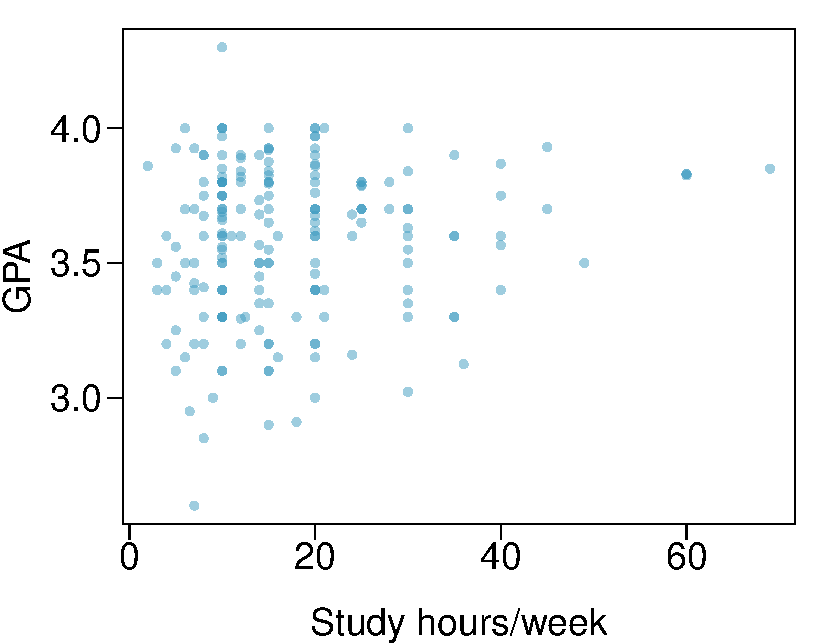
\includegraphics[width = 0.78\textwidth]{ch_data_collection/figures/eoce/gpaStudy/gpaStudy}
\end{center}
\end{minipage}
}{}


% 12

\eoce{\qt{Income and education} The scatterplot below shows the relationship between per capita income (in thousands of dollars) and percent of population with a bachelor's degree in 3,143 counties in the US in 2010.

\noindent\begin{minipage}[c]{0.44\textwidth}
\begin{parts}
\item What are the explanatory and response variables?
\item Describe the relationship between the two variables. Make sure to discuss unusual observations, if any.
\item Can we conclude that having a bachelor's degree increases one's income?
\end{parts} \textA{\vspace{16mm}}
\end{minipage}
\begin{minipage}[c]{0.55\textwidth}
\begin{center}
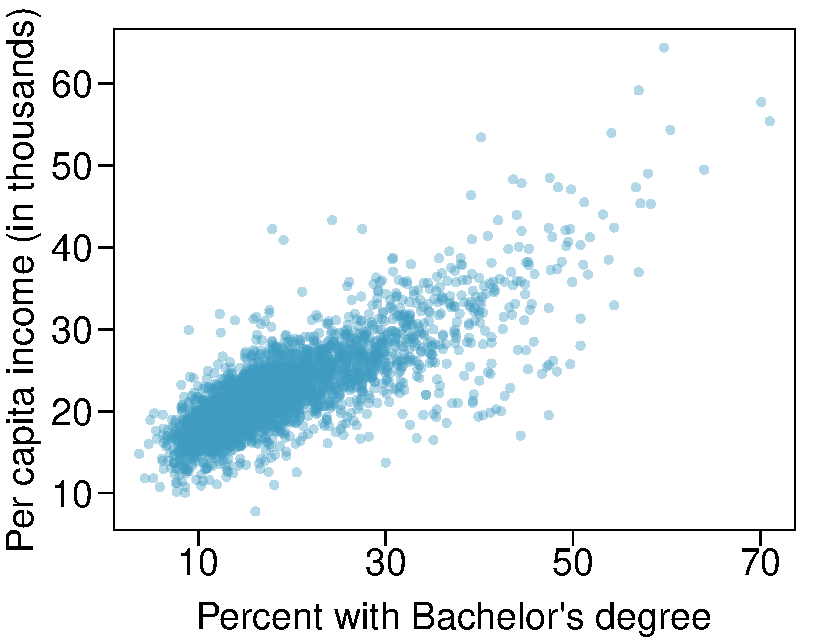
\includegraphics[width = 0.78\textwidth]{ch_data_collection/figures/eoce/county/county_incomeBach}
\end{center}
\end{minipage}
}{}


%_________________
\subsection{Observational studies and sampling strategies}
% 1.6.4

% 13

\eoce{\qt{Propose a sampling strategy, Part I} A large college class has 160 students. All 160 students attend the lectures together, but the students are divided into 4 groups, each of 40 students, for lab sections administered by different teaching assistants. The professor wants to conduct a survey about how satisfied the students are with the course, and he believes that the lab section a student is in might affect the student's overall satisfaction with the course.
\begin{parts}
\item What type of study is this?
\item Suggest a sampling strategy for carrying out this study.
\end{parts}
}{}

% 14

\eoce{\qt{Propose a sampling strategy, Part II} On a large college campus first-year students and sophomores live in dorms located on the eastern part of the campus and juniors and seniors live in dorms located on the western part of the campus. Suppose you want to collect student opinions on a new housing structure the college administration is proposing and you want to make sure your survey equally represents opinions from students from all years.
\begin{parts}
\item What type of study is this?
\item Suggest a sampling strategy for carrying out this study.
\end{parts}
}{}

% 15

\eoce{\qt{Internet use and life expectancy} The scatterplot below shows the relationship between estimated life expectancy at birth as of 2012\footfullcite{data:ciaFactBookLifeExp:2012} and percentage of internet users in 2010\footfullcite{data:ITU:2012} in 208 countries.

\noindent\begin{minipage}[c]{0.43\textwidth}
\begin{parts}
\item Describe the relationship between life expectancy and percentage of internet users.
\item What type of study is this?
\item State a possible confounding variable that might explain this relationship and describe its potential effect.
\end{parts}\vspace{16mm}
\end{minipage}%
\begin{minipage}[r]{0.55\textwidth}
\hfill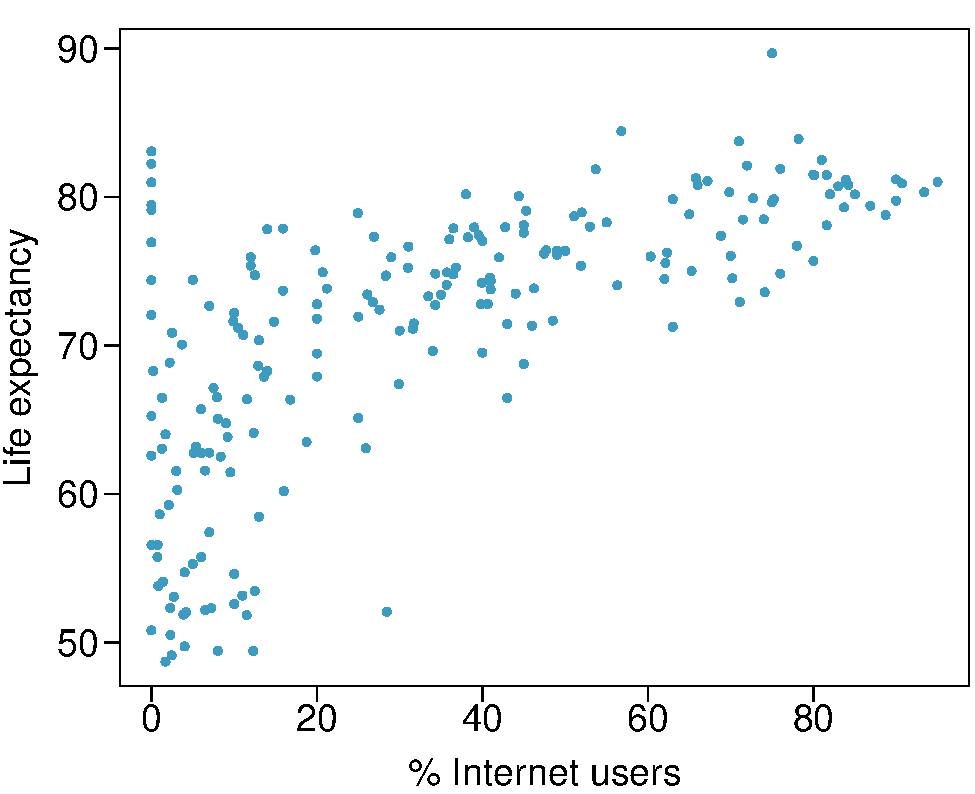
\includegraphics[width = 0.95\textwidth]{ch_data_collection/figures/eoce/country/county_lifeExpInter}
\end{minipage}
}{}

% 16

\eoce{\qt{Stressed out, Part I} A study that surveyed a random sample of otherwise healthy high school students found that they are more likely to get muscle cramps when they are stressed. The study also noted that students drink more coffee and sleep less when they are stressed.
\begin{parts}
\item What type of study is this?
\item Can this study be used to conclude a causal relationship between increased stress and muscle cramps?
\item State possible confounding variables that might explain the observed relationship between increased stress and muscle cramps. 
\end{parts}
}{}

% 17

\eoce{\qt{Random digit dialing} The Gallup Poll uses a procedure called random digit dialing, which creates phone numbers based on a list of all area codes in America in conjunction with the associated number of residential households in each area code. Give a possible reason the Gallup Poll chooses to use random digit dialing instead of picking phone numbers from the phone book.
}{}

% 18

\eoce{\qt{Haters are gonna hate, study confirms} A study published in the \textit{Journal of Personality and Social Psychology} asked a group of 200 randomly sampled men and women to evaluate how they felt about various subjects, such as camping, health care, architecture, taxidermy, crossword puzzles, and Japan in order to measure their dispositional attitude towards mostly independent stimuli. Then, they presented the participants with information about a new product: a microwave oven. This microwave oven does not exist, but the participants didn't know this, and were given three positive and three negative fake reviews. People who reacted positively to the subjects on the dispositional attitude measurement also tended to react positively to the microwave oven, and those who reacted negatively also tended to react negatively to it. Researchers concluded that ``some people tend to like things, whereas others tend to dislike things, and a more thorough understanding of this tendency will lead to a more thorough understanding of the psychology of attitudes." \footfullcite{Hepler:2013}
\begin{parts}
\item What are the cases?
\item What is (are) the response variable(s) in this study?
\item What is (are) the explanatory variable(s) in this study?
\item Does the study employ random sampling?
\item Is this an observational study or an experiment? Explain your reasoning.
\item Can we establish a causal link between the explanatory and response variables?
\item Can the results of the study be generalized to the population at large?
\end{parts}
}{}


% 19

\eoce{\qt{Family size} Suppose we want to estimate household size, where a ``household" is defined as people living together in the same dwelling, and sharing living accommodations. If we select students at random at an elementary school and ask them what their family size is, will this be a good measure of household size? Or will our average be biased? If so, will it overestimate or underestimate the true value?
}{}

% 20

\eoce{\qt{Flawed reasoning} Identify the flaw(s) in reasoning in the following scenarios. Explain what the individuals in the study should have done differently if they wanted to make such strong conclusions.
\begin{parts}
\item Students at an elementary school are given a questionnaire that they are asked to return after their parents have completed it. One of the questions asked is, ``Do you find that your work schedule makes it difficult for you to spend time with your kids after school?" Of the parents who replied, 85\% said ``no". Based on these results, the school officials conclude that a great majority of the parents have no difficulty spending time with their kids after school.
\item A survey is conducted on a simple random sample of 1,000 women who recently gave birth, asking them about whether or not they smoked during pregnancy. A follow-up survey asking if the children have respiratory problems is conducted 3 years later, however, only 567 of these women are reached at the same address. The researcher reports that these 567 women are representative of all mothers.
\item An orthopedist administers a questionnaire to 30 of his patients who do not have any joint problems and finds that 20 of them regularly go running. He concludes that running decreases the risk of joint problems.
\end{parts}
}{}

% 21

\eoce{\qt{City council survey} A city council has requested a household survey be conducted in a suburban area of their city. The area is broken into many distinct and unique neighborhoods, some including large homes, some with only apartments, and others a diverse mixture of housing structures. Identify the sampling methods described below, and comment on whether or not you think they would be effective in this setting.
\begin{parts}
\item Randomly sample 50 households from the city.
\item Divide the city into neighborhoods, and sample 20 households from each neighborhood.
\item Divide the city into neighborhoods, randomly sample 10 neighborhoods, and sample all households from those neighborhoods.
\item Divide the city into neighborhoods, randomly sample 10 neighborhoods, and then randomly sample 20 households from those neighborhoods.
\item Sample the 200 households closest to the city council offices.
\end{parts}
}{}


\textA{\pagebreak}

% 22

\eoce{\qt{Sampling strategies} A statistics student who is curious about the relationship between the amount of time students spend on social networking sites and their performance at school decides to conduct a survey. Various research strategies for collecting data are described below. In each, name the sampling method proposed and any bias you might expect.
\begin{parts}
\item He randomly samples 40 students from the study's population, gives them the survey, asks them to fill it out and bring it back the next day.
\item He gives out the survey only to his friends, making sure each one of them fills out the survey.
\item He posts a link to an online survey on Facebook and asks his friends to fill out the survey.
\item He randomly samples 5 classes and asks a random sample of students from those classes to fill out the survey.
\item He stands outside the student center and asks every third person that walks out the door to fill out the survey.
\end{parts}
}{}

% 23

\eoce{\qt{Reading the paper} Below are excerpts from two articles published in the \emph{NY Times}:
\begin{parts}
\item An article titled \emph{Risks: Smokers Found More Prone to Dementia} states the following: \footfullcite{news:smokingDementia}
\begin{adjustwidth}{1em}{1em}
{\footnotesize ``Researchers analyzed data from 23,123 health plan members who participated in a voluntary exam and health behavior survey from 1978 to 1985, when they were 50-60 years old. 23 years later, about 25\% of the group had dementia, including 1,136 with Alzheimer�s disease and 416 with vascular dementia. After adjusting for other factors, the researchers concluded that pack-a-day smokers were 37\% more likely than nonsmokers to develop dementia, and the risks went up with increased smoking; 44\% for one to two packs a day; and twice the risk for more than two packs."}
\end{adjustwidth}
Based on this study, can we conclude that smoking causes dementia later in life? Explain your reasoning.
\item Another article titled \emph{The School Bully Is Sleepy} states the following: \footfullcite{news:bullySleep}
\begin{adjustwidth}{1em}{1em}
{\footnotesize ``The University of Michigan study, collected survey data from parents on each child's sleep habits and asked both parents and teachers to assess behavioral concerns. About a third of the students studied were identified by parents or teachers as having problems with disruptive behavior or bullying. The researchers found that children who had behavioral issues and those who were identified as bullies were twice as likely to have shown symptoms of sleep disorders."}
\end{adjustwidth}
A friend of yours who read the article says, ``The study shows that sleep disorders lead to bullying in school children." Is this statement justified? If not, how best can you describe the conclusion that can be drawn from this study?
\end{parts}
}{}

% 24

\eoce{\qt{Shyness on Facebook} Given the anonymity afforded to individuals in online interactions, researchers hypothesized that shy individuals might have more favorable attitudes toward Facebook, and that shyness might be positively correlated with time spent on Facebook. They also hypothesized that shy individuals might have fewer Facebook ``friends" as they tend to have fewer friends than non-shy individuals have in the offline world. 103 undergraduate students at an Ontario university were surveyed via online questionnaires. The study states ``Participants were recruited through the university's psychology participation pool. After indicating an interest in the study, participants were sent an e-mail containing the study's URL." Are the results of this study generalizable to the population of all Facebook users? \footfullcite{Orr:2009}
}{}


\textA{\pagebreak}


%_________________
\subsection{Experiments}
% 1.6.5

% 25
\eoce{\qt{Stressed out, Part II} In a study evaluating the relationship between stress and muscle cramps, half the subjects are randomly assigned to be exposed to increased stress by being placed into an elevator that falls rapidly and stops abruptly and the other half are left at no or baseline stress.
\begin{parts}
\item What type of study is this?
\item Can this study be used to conclude a causal relationship between increased stress and muscle cramps?
\end{parts}
}{}

% 26
\eoce{\qt{Light and exam performance} A study is designed to test the effect of light level on exam performance of students. The researcher believes that light levels might have different effects on males and females, so wants to make sure both are equally represented in each treatment. The treatments are fluorescent overhead lighting, yellow overhead lighting, no overhead lighting (only desk lamps). 
\begin{parts}
\item What is the response variable?
\item What is the explanatory variable? What are its levels?
\item What is the blocking variable? What are its levels?
\end{parts}
}{}

% 27

\eoce{\qt{Vitamin supplements} In order to assess the effectiveness of taking large doses of vitamin C in reducing the duration of the common cold, researchers recruited 400 healthy volunteers from staff and students at a university. A quarter of the patients were assigned a placebo, and the rest were evenly divided between 1g Vitamin C,  3g Vitamin C, or 3g Vitamin C plus additives to be taken at onset of a cold for the following two days. All tablets had identical appearance and packaging. The nurses who handed the prescribed pills to the patients knew which patient received which treatment, but the researchers assessing the patients when they were sick did not. No significant differences were observed in any measure of cold duration or severity between the four medication groups, and the placebo group had the shortest duration of symptoms.\footfullcite{Audera:2001}
\begin{parts}
\item Was this an experiment or an observational study? Why?
\item What are the explanatory and response variables in this study?
\item Were the patients blinded to their treatment?
\item Was this study double-blind?
\item Participants are ultimately able to choose whether or not to use the pills prescribed to them. We might expect that not all of them will adhere and take their pills. Does this introduce a confounding variable to the study? Explain your reasoning.
\end{parts}
}{}


% 28
\eoce{\qt{Light, noise, and exam performance} A study is designed to test the effect of light level and noise level on exam performance of students. The researcher believes that light and noise levels might have different effects on males and females, so wants to make sure both are equally represented in each treatment. The light treatments considered are fluorescent overhead lighting, yellow overhead lighting, no overhead lighting (only desk lamps). The noise treatments considered are no noise,  construction noise, and human chatter noise.
\begin{parts}
\item What is the response variable?
\item How many factors are considered in this study? Identify them, and describe their levels.
\item What is the role of the sex variable in this study?
\end{parts}
}{}

% 29
\eoce{\qt{Music and learning} You would like to conduct an experiment in class to see if students learn better if they study without any music, with music that has no lyrics (instrumental), or with music that has lyrics. Briefly outline a design for this study.
}{}

% 30

\eoce{\qt{Soda preference} You would like to conduct an experiment in class to see if your classmates prefer the taste of regular Coke or Diet Coke. Briefly outline a design for this study.
}{}

% 31

\eoce{\qt{Exercise and mental health} A researcher is interested in the effects of exercise on mental health and he proposes the following study: Use stratified random sampling to ensure representative proportions of 18-30, 31-40 and 41-55 year olds from the population. Next, randomly assign half the subjects from each age group to exercise twice a week, and instruct the rest not to exercise. Conduct a mental health exam at the beginning and at the end of the study, and compare the results.
\begin{parts}
\item What type of study is this? 
\item What are the treatment and control groups in this study?
\item Does this study make use of blocking? If so, what is the blocking variable?
\item Does this study make use of blinding?
\item Comment on whether or not the results of the study can be used to establish a causal relationship between exercise and mental health, and indicate whether or not the conclusions can be generalized to the population at large.
\item Suppose you are given the task of determining if this proposed study should get funding. Would you have any reservations about the study proposal?
\end{parts}
}{}

% 32

\eoce{\qt{Chia seeds and weight loss} Chia Pets -- those terra-cotta figurines that sprout fuzzy green hair -- made the chia plant a household name. But chia has gained an entirely new reputation as a diet supplement.  In one 2009 study, a team of researchers recruited 38 men and divided them randomly into two groups: treatment or control. They also recruited 38 women, and they randomly placed half of these participants into the treatment group and the other half into the control group. One group was given 25 grams of chia seeds twice a day, and the other was given a placebo. The subjects volunteered to be a part of the study. After 12 weeks, the scientists found no significant difference between the groups in appetite or weight loss. \footfullcite{Nieman:2009}
\begin{parts}
\item What type of study is this? 
\item What are the experimental and control treatments in this study?
\item Has blocking been used in this study? If so, what is the blocking variable?
\item Has blinding been used in this study?
\item Comment on whether or not we can make a causal statement, and indicate whether or not we can generalize the conclusion to the population at large.
\end{parts}
}{}

% 33

\eoce{\qt{Multitaskers, Part I} Researchers studying the effect of TV watching while studying on school performance conducted the following studies. For each study determine (i) the type of study (observational or experiment), (ii) if there is random sampling, (iii) if there is random assignment, (iv) state the scope of the conclusions of the study, and (v) note if stratifying, blocking, or neither of these techniques were used in the study.
\begin{parts}
\item Researchers randomly sampled 100 high school students and asked them whether or not they watched TV while studying. They found that the mean grade point average of students who did not watch TV while studying was significantly higher than the mean grade point average of students who did watch TV while studying.
\item Researchers randomly sampled 50 female and 50 male high school students and asked them whether or not they watched TV while studying. They found that the mean grade point average of both males and females who did not watch TV while doing homework was significantly higher than the mean grade point average of students who did watch TV while doing homework. \textA{\textbf{(Note that there is a part~(c) on the next page.)}}
\item Researchers randomly sampled 100 high school students and randomly assigned them into two study groups. Throughout the school year, one group was told to study in a room with a TV on while the other was told to study in silence. At the end of the year the researchers compared the grade point averages of the two groups and found that the mean grade point average of students who did not watch TV while studying was significantly higher than the grade point average of students who did watch TV while studying.
\end{parts}
}{}

% 34
\eoce{\qt{Multitaskers, Part II} Researchers investigating the effect of studying while watching TV on school performance conducted the following studies. For each study determine (i) the type of study (observational or experiment), (ii) if there is random sampling, (iii) if there is random assignment, (iv) state the scope of the conclusions of the study, and (v) note if stratifying, blocking, or neither of these techniques were used in the study.
\begin{parts}
\item Researchers randomly sampled 50 female and 50 male high school students. Half of the females and half of the males were randomly assigned to study in a room with a TV and the remainder studied without a TV. They found that the mean grade point average of both males and females who did not watch TV while studying was significantly higher than those who did watch TV while studying.
\item Researchers surveyed the first 100 students who showed up to prom. They found that the mean grade point average of students who did not watch TV while studying was higher than the mean grade point average for students who did watch TV while studying.
\item Researchers surveyed the first 50 male and 50 female students who showed up to prom. They found that the mean grade point average of both males and females who did not watch TV while doing homework was higher than the mean grade point average of students who did watch TV while studying.
\end{parts}
}{}


% 35

\eoce{\qt{Multitaskers, Part III} Suppose a friend of yours wants to design his own study for evaluating the effect of TV watching on school performance. He proposes comparing the grade point averages of everyone in his homeroom class who do and do not watch TV while doing homework, and extending the results of this study to draw conclusions about all high schoolers. Indicate any mistakes with this design, keeping in mind that the goal of the study is to assess the causal relationship between TV watching and school performance for high schoolers.
}{}

% 36

\eoce{\qt{Multitaskers, Part IV} Suppose two friends of yours want to design their own study for evaluating the effect of TV watching on school performance. They propose the following designs. Indicate any mistakes with these designs, keeping in mind that the goal of the study is to assess the causal relationship between TV watching and school performance for high schoolers.
\begin{parts}
\item Randomly sample 100 students from the entire school. Reserve two classrooms for a study session and the first 50 people that show up get assigned to the room where the TV will be on and the rest to the room where they can study in silence for a final exam. Then compare the average grades of the two groups at the end of the semester.
\item Age and involvement in extracurricular activities may be factors that affect the academic performance of a student, so these characteristics should be blocked for when studying the effect of watching TV while studying. To achieve this aim, sample 10 first-years, 10 sophomores, 10 juniors, and 10 seniors, 5 of which are heavily involved with extracurricular activities and 5 of which are not from each class. Then ask them whether they watch TV while they study, and compare the average GPAs of those who do and do not.
\end{parts}
}{}

% 37
\eoce{\qt{Running on electrolytes} Suppose you would like to design a study evaluating whether consuming a sports drink that replenishes electrolytes can make you run faster. You were able to recruit 50 students to participate in your study. Describe how you can use matched pairs design and blinding for this study.}
{}

\textA{\pagebreak}

% 38
\eoce{\qt{Improving life satisfaction} In a study evaluating the effectiveness of a positive psychology group intervention, forty middle schoolers who were identified as being less than delighted with their lives (reported life satisfaction scores between 1 and 6 on a 7-point scale) were randomly assigned to receive the intervention (treatment) or not receive the intervention (control). These students were first matched on attributes such as sex, socioeconomic group, race/ethnicity, and age, such that each student in the treatment group had a matched counterpart in the control group. Researchers found that life satisfaction of students in the intervention group increased significantly,  while the control group declined during the same period (although this change was not statistically significant). \footfullcite{Suldo:2014}
\begin{parts}
\item What type of study is this?
\item What type of design is used in this study?
\item Can the results of this study be used to establish a causal link between the intervention and increased life satisfaction in middle schoolers?
\end{parts}
}{}


% 39

\eoce{\qt{Alfalfa plants} Researchers were interested in the effect that acid has on the growth rate of alfalfa plants. They created three treatment groups in an experiment: low acid ($+$), high acid ($\triangle$), and control ($\ocircle$). The alfalfa plants were grown in a Styrofoam cups arranged near a window and the height of the alfalfa plants was measured after five days of growth. The experiment consisted of 6 cups for each of the 3 treatments, for a total of 18 observations. Which of the following designs is preferable? Note that the dotted line indicates the location of the window. Explain your reasoning.
\begin{center}
\begin{minipage}[c]{0.3\textwidth}
\begin{center}
Design A \\
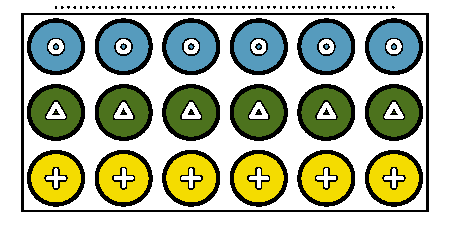
\includegraphics[width = \textwidth]{ch_data_collection/figures/eoce/alfalfa/alfalfaA}
\end{center}
\end{minipage}
\begin{minipage}[c]{0.3\textwidth}
\begin{center}
Design B \\
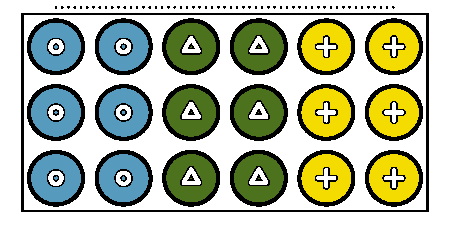
\includegraphics[width = \textwidth]{ch_data_collection/figures/eoce/alfalfa/alfalfaB}
\end{center}
\end{minipage}
\begin{minipage}[c]{0.3\textwidth}
\begin{center}
Design C \\
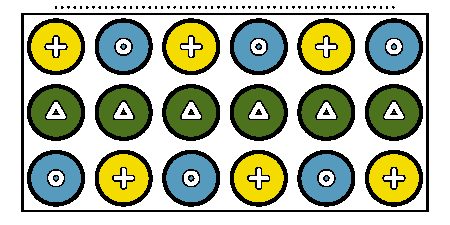
\includegraphics[width = \textwidth]{ch_data_collection/figures/eoce/alfalfa/alfalfaC}
\end{center}
\end{minipage}
\end{center}
}{}

% 40

\eoce{\qt{Chocolate chip cookies} We would like to compare two cookie recipes, one from a popular recipe website and another from the back of a bag of chocolate chips. We will bake 24 cookies, 12 of each type, and then have a friend rate each cookie on a scale of 1 to 10. Both sets of cookies are supposed to be baked for the same amount of time and at the same temperature: 9 minutes at 350F. We will use an old oven available to students in the school, which tends to overheat a little near the oven's back.
\begin{parts}
\item Would we bias our results if we cooked one type of cookie first and the other second?
\item We instead decide to bake each batch simultaneously on the same tray, and decide to block for proximity to the back of the oven. Two blocking schemes shown below are under consideration. For each scheme, cookies made with the recipe from the website are indicated with a $+$ and cookies made with the other recipe are indicated with a $\ocircle$. The dashed line marks the back of the oven. Which of the blocking schemes, A or B, is better for this experiment? Explain your answer.
\begin{center}
\begin{minipage}[c]{0.35\textwidth}
\begin{center}
Blocking scheme A \\
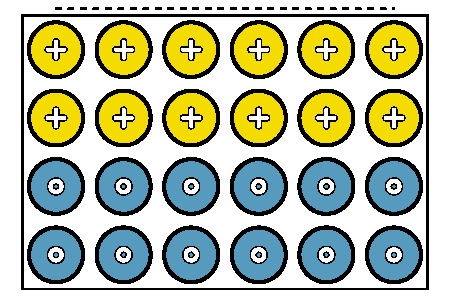
\includegraphics[width = 0.81\textwidth]{ch_data_collection/figures/eoce/cookies/cookiesA}
\end{center}
\end{minipage}
\begin{minipage}[c]{0.35\textwidth}
\begin{center}
Blocking scheme B \\
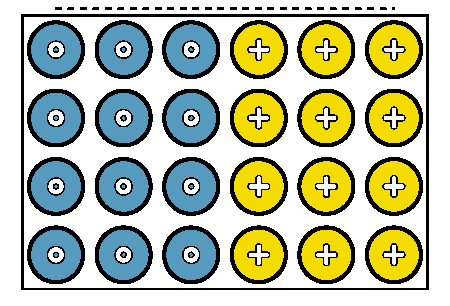
\includegraphics[width = 0.81\textwidth]{ch_data_collection/figures/eoce/cookies/cookiesB}
\end{center}
\end{minipage}
\end{center}
\item How can the blocking scheme you chose in the previous part be improved?
\end{parts}
}{}













